\documentclass[12pt,a4paper]{article}
\usepackage[utf8]{inputenc}
\usepackage{amsmath}
\usepackage{amsfonts}
\usepackage{amssymb}
\usepackage{graphicx}
\usepackage{float}
\usepackage{hyperref}
\usepackage{geometry}
\usepackage{xcolor}
\usepackage{listings}
\usepackage{booktabs}

\geometry{margin=1in}
\hypersetup{
    colorlinks=true,
    linkcolor=blue,
    filecolor=magenta,      
    urlcolor=cyan,
    pdftitle={Problem Set 3 Solutions},
    pdfpagemode=FullScreen,
}

\begin{document}

\begin{abstract}
This report presents the solutions to Problem Set 3, focusing on finite element analysis for one-dimensional elements. The problems involve shape functions, displacements, strains, and stiffness matrices for 2-node and 3-node elements.
\end{abstract}

\section{Introduction}
Finite Element Analysis (FEA) is a numerical method for solving engineering problems involving complex geometries, loadings, and material properties. In this report, we apply FEA principles to solve two problems involving 2-node and 3-node elements. For each problem, we derive shape functions, calculate displacements and strains at specific points, and compute element stiffness matrices.

\section{Problem 1: Three 2-Node Elements}

Consider a structure consisting of three 2-node elements with nodes at $x = 0, 2, 4, 6$. The displacements at nodes 1, 2, 3, and 4 are 1, 3, 4, and 6 respectively.

\begin{figure}[H]
\centering
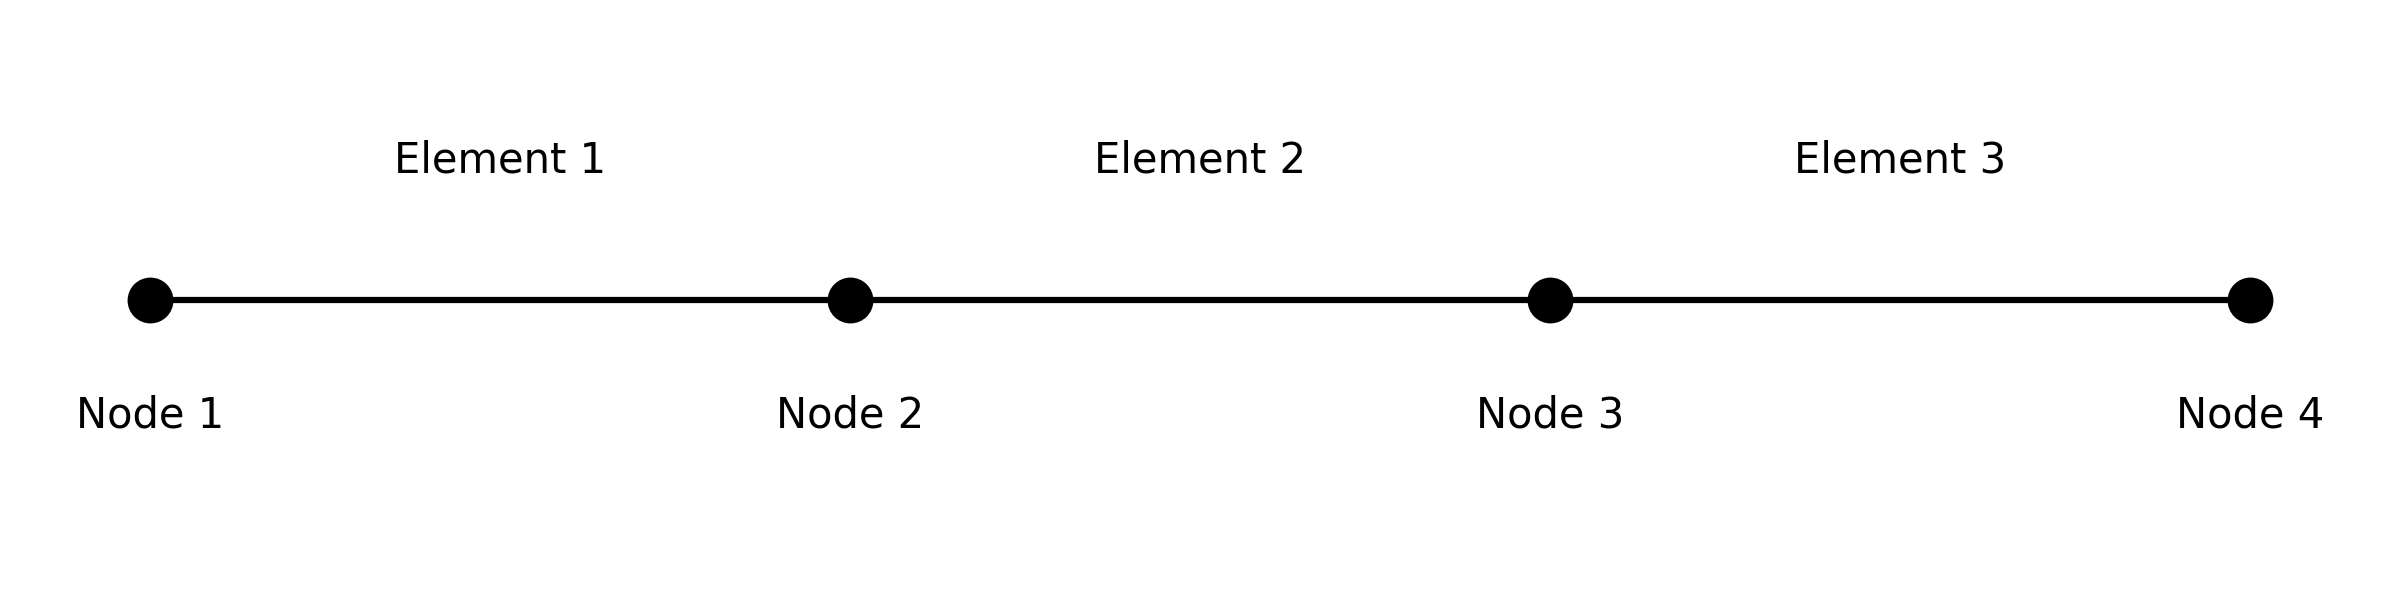
\includegraphics[width=0.8\textwidth]{figures/problem1_structure.png}
\caption{Problem 1: Structure with three 2-node elements}
\label{fig:problem1_structure}
\end{figure}

\subsection{Shape Functions}
For 2-node elements, the shape functions are:
\begin{align}
N_1(\xi) &= \frac{1-\xi}{2} \\
N_2(\xi) &= \frac{1+\xi}{2}
\end{align}
where $\xi$ is the local coordinate ranging from -1 to 1 within each element.

\subsection{Displacements at $\xi = 0.5$}
The displacement at $\xi = 0.5$ in each element is calculated using the shape functions:
\begin{equation}
u(\xi) = N_1(\xi)u_1 + N_2(\xi)u_2
\end{equation}

For $\xi = 0.5$:
\begin{align}
N_1(0.5) &= \frac{1-0.5}{2} = 0.25 \\
N_2(0.5) &= \frac{1+0.5}{2} = 0.75
\end{align}

\subsubsection*{Element 1 (nodes 1-2):}
\begin{align}
u(\xi=0.5) &= 0.25 \times 1 + 0.75 \times 3 \\
&= 0.25 + 2.25 = 2.5
\end{align}

\subsubsection*{Element 2 (nodes 2-3):}
\begin{align}
u(\xi=0.5) &= 0.25 \times 3 + 0.75 \times 4 \\
&= 0.75 + 3.0 = 3.75
\end{align}

\subsubsection*{Element 3 (nodes 3-4):}
\begin{align}
u(\xi=0.5) &= 0.25 \times 4 + 0.75 \times 6 \\
&= 1.0 + 4.5 = 5.5
\end{align}

\begin{figure}[H]
\centering
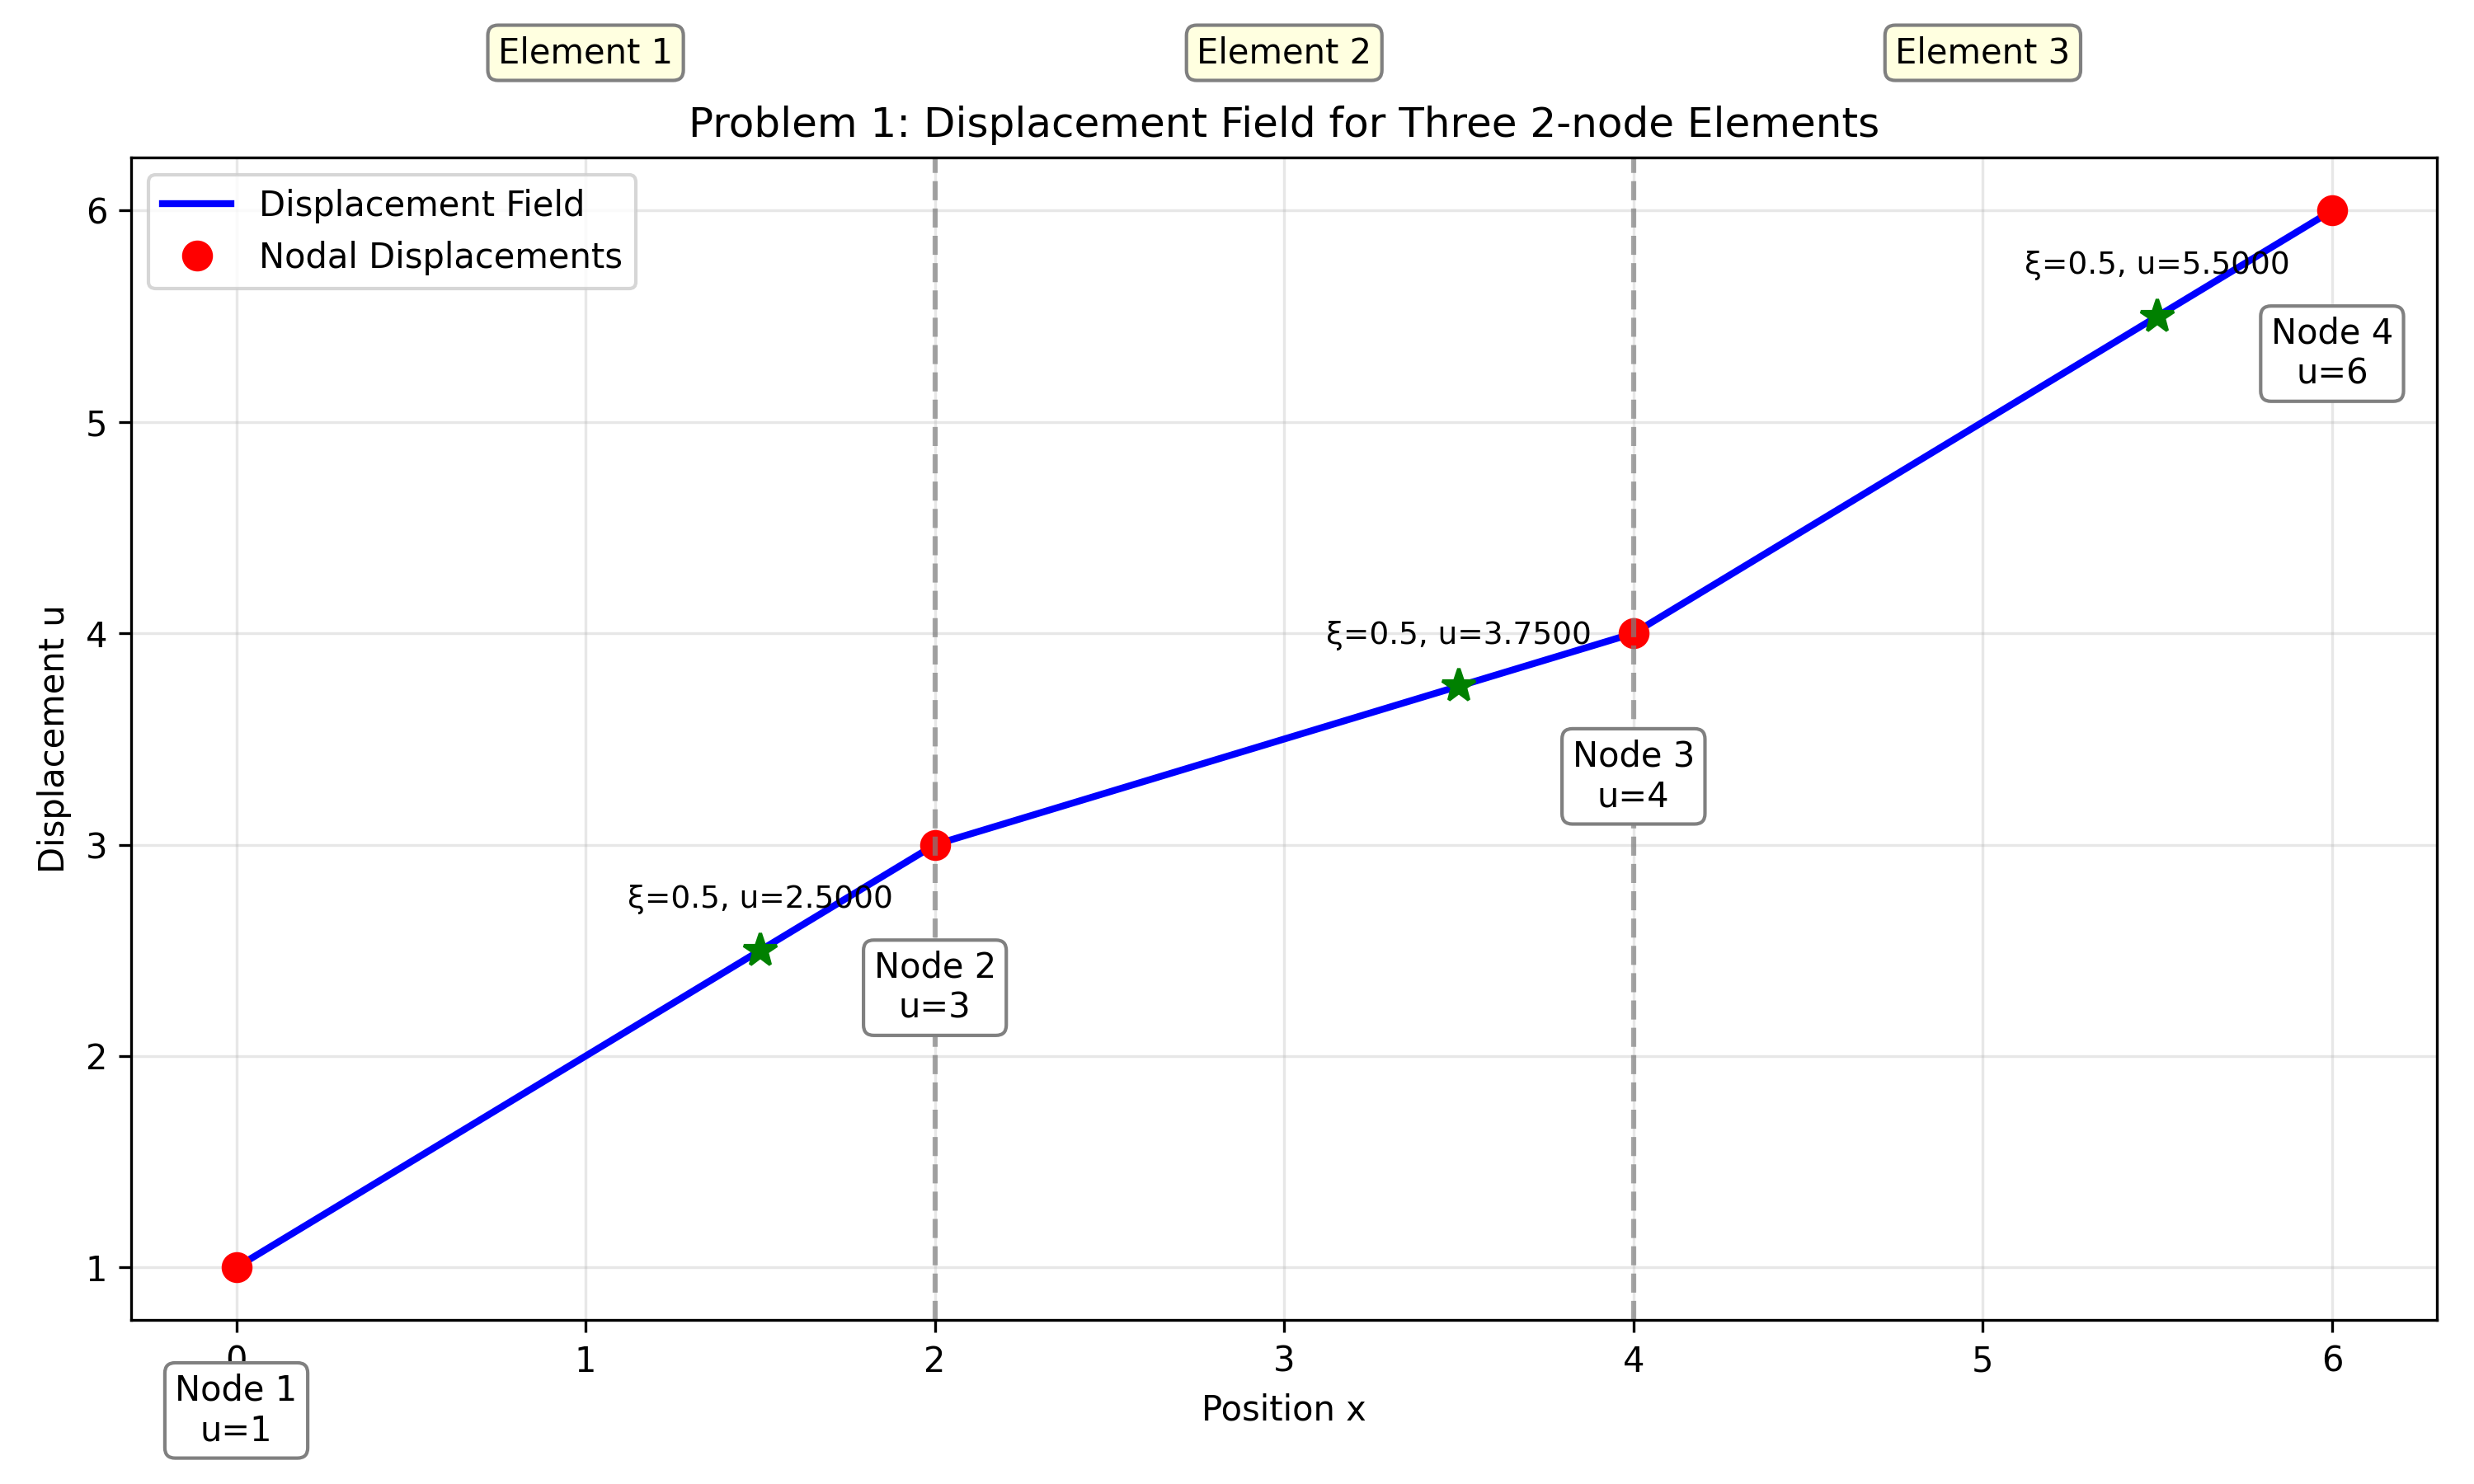
\includegraphics[width=0.8\textwidth]{figures/ps3_problem1_displacement.png}
\caption{Problem 1: Displacement field for the three 2-node elements}
\label{fig:problem1_displacement}
\end{figure}

\subsection{Strains at $\xi = 0.5$}
For 2-node elements, the strain is constant throughout the element:
\begin{equation}
\varepsilon = \frac{u_2 - u_1}{L}
\end{equation}

\subsubsection*{Element 1 (L = 2):}
\begin{align}
\varepsilon &= \frac{3 - 1}{2} = 1.0
\end{align}

\subsubsection*{Element 2 (L = 2):}
\begin{align}
\varepsilon &= \frac{4 - 3}{2} = 0.5
\end{align}

\subsubsection*{Element 3 (L = 2):}
\begin{align}
\varepsilon &= \frac{6 - 4}{2} = 1.0
\end{align}

\begin{figure}[H]
\centering
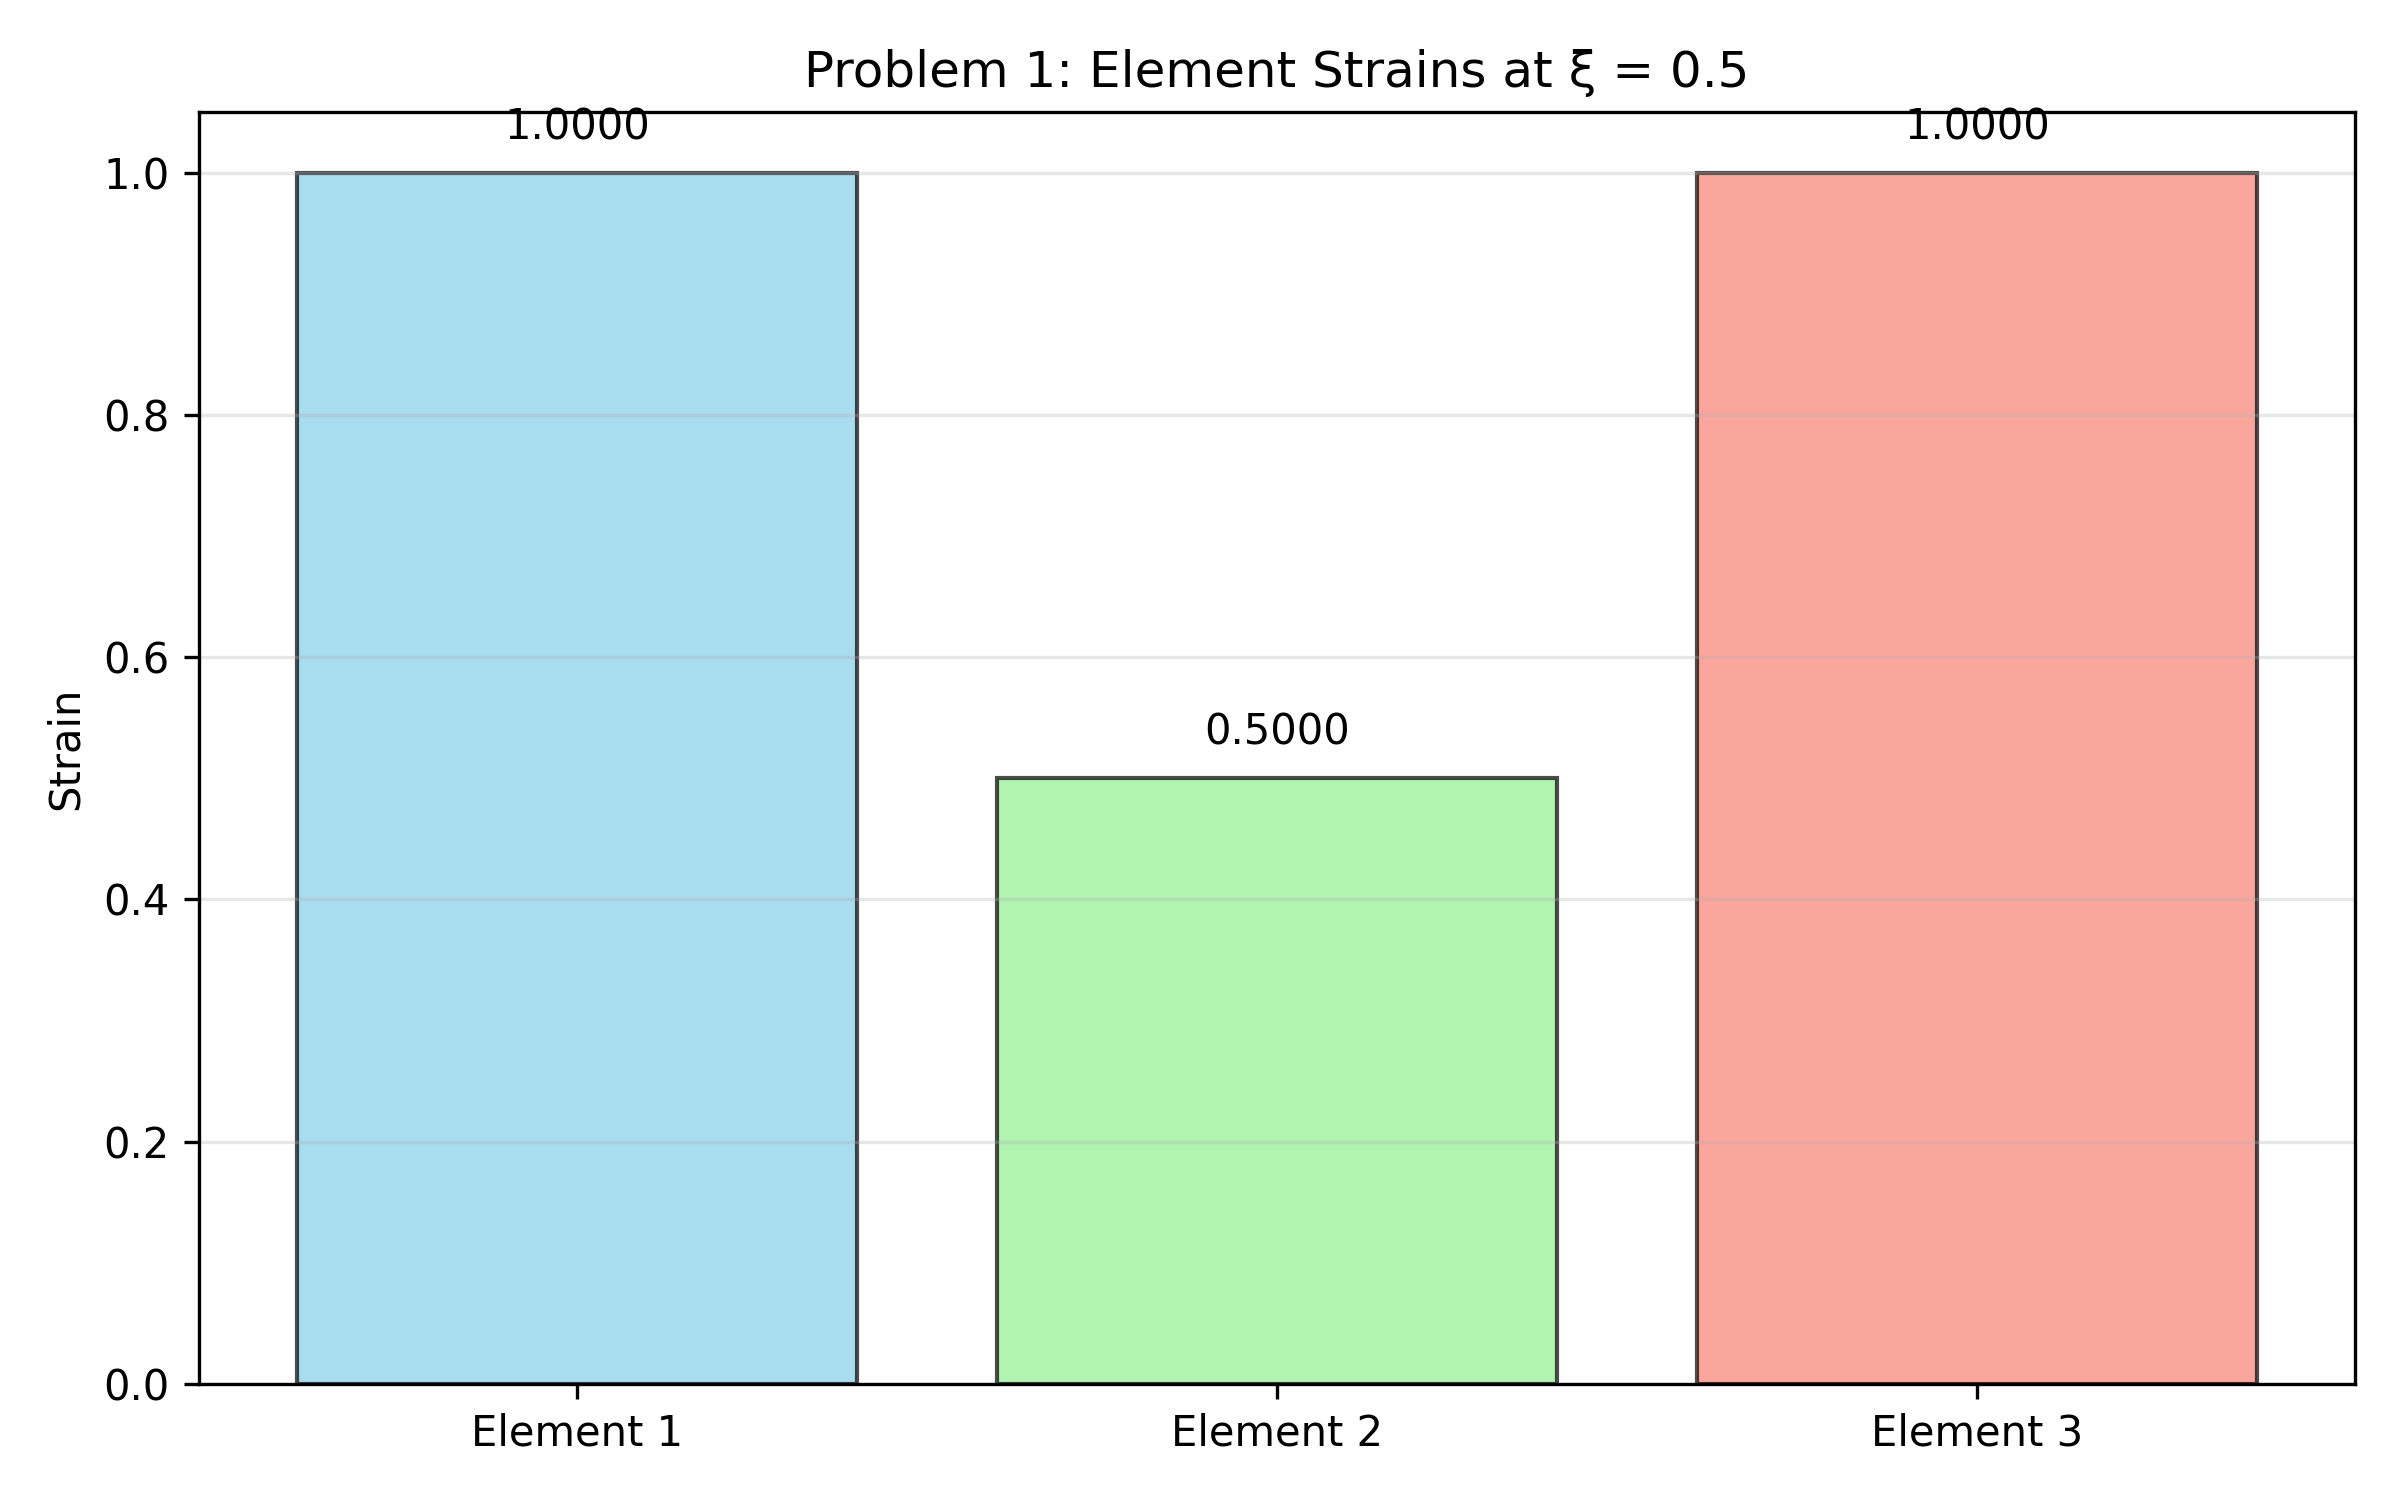
\includegraphics[width=0.8\textwidth]{figures/ps3_problem1_strains.png}
\caption{Problem 1: Element strains for the three 2-node elements}
\label{fig:problem1_strains}
\end{figure}

\subsection{Stiffness Matrices}
For a 2-node element with Young's modulus $E$ and cross-sectional area $A$, the stiffness matrix is:
\begin{equation}
\mathbf{k} = \frac{E \cdot A}{L} \begin{bmatrix} 1 & -1 \\ -1 & 1 \end{bmatrix}
\end{equation}

Assuming $E = A = 1$ for simplicity:

\subsubsection*{Element 1 (L = 2):}
\begin{align}
\mathbf{k_1} &= \frac{1 \cdot 1}{2} \begin{bmatrix} 1 & -1 \\ -1 & 1 \end{bmatrix} \\
&= 0.5 \begin{bmatrix} 1 & -1 \\ -1 & 1 \end{bmatrix} \\
&= \begin{bmatrix} 0.5 & -0.5 \\ -0.5 & 0.5 \end{bmatrix}
\end{align}

\subsubsection*{Element 2 (L = 2):}
\begin{align}
\mathbf{k_2} &= 0.5 \begin{bmatrix} 1 & -1 \\ -1 & 1 \end{bmatrix} \\
&= \begin{bmatrix} 0.5 & -0.5 \\ -0.5 & 0.5 \end{bmatrix}
\end{align}

\subsubsection*{Element 3 (L = 2):}
\begin{align}
\mathbf{k_3} &= 0.5 \begin{bmatrix} 1 & -1 \\ -1 & 1 \end{bmatrix} \\
&= \begin{bmatrix} 0.5 & -0.5 \\ -0.5 & 0.5 \end{bmatrix}
\end{align}

\section{Problem 2: Two 3-Node Elements}

Consider a structure consisting of two 3-node elements with nodes at $x = 0, 2, 4, 6, 8$. The displacements at nodes 1, 2, 3, 4, and 5 are 0, -1, 2, -1, and 4 respectively. Element 1 connects nodes 1, 2, and 3, while Element 2 connects nodes 3, 4, and 5.

\begin{figure}[H]
\centering
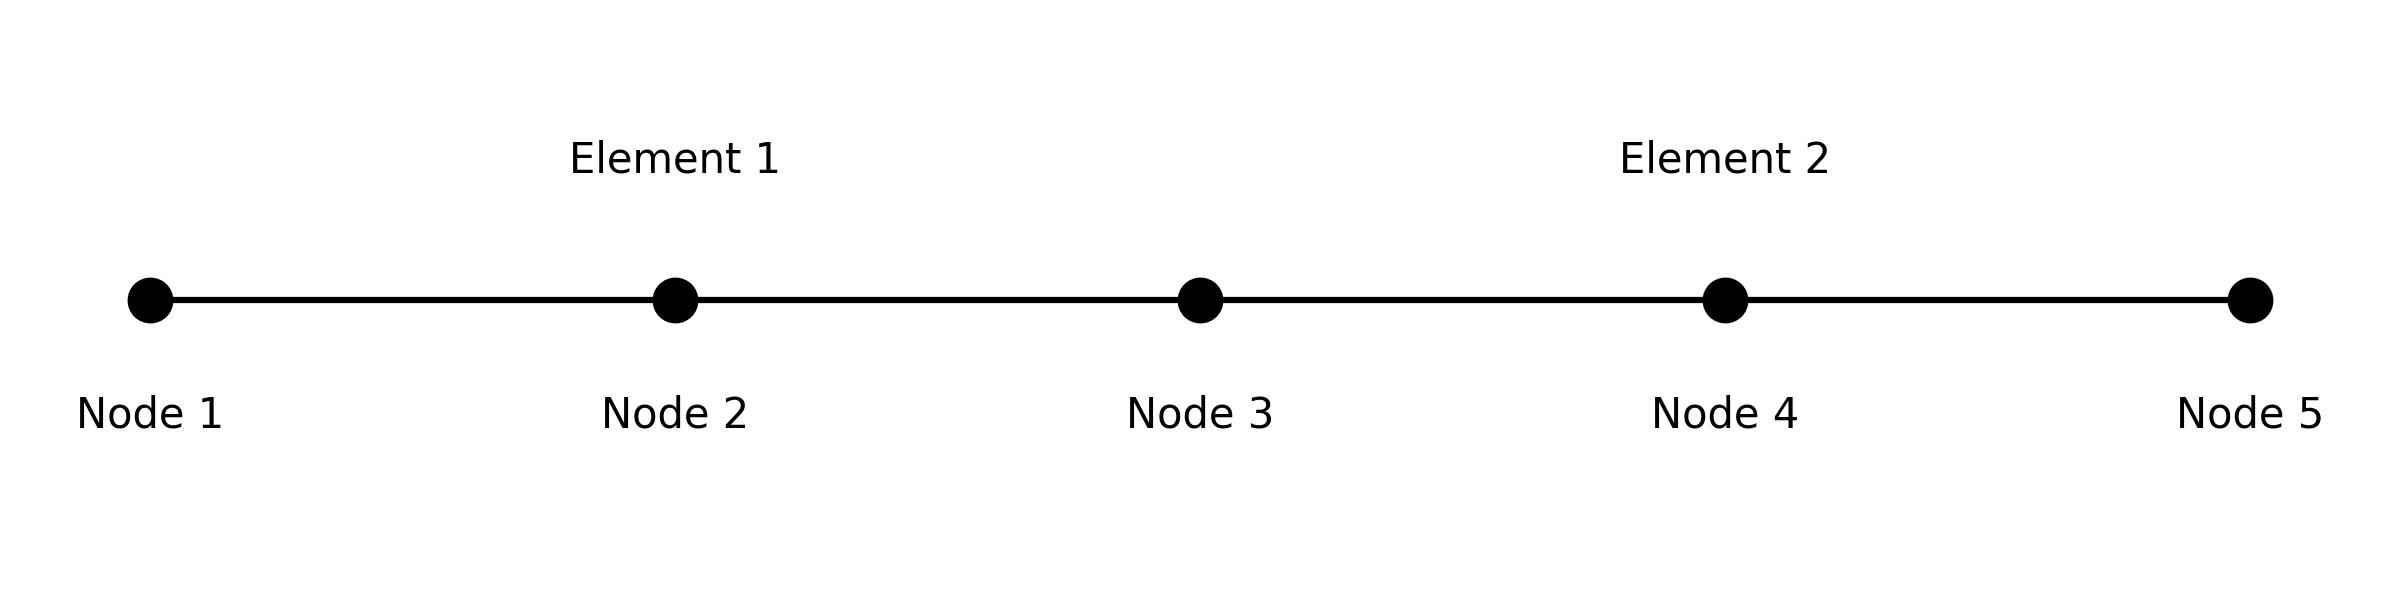
\includegraphics[width=0.8\textwidth]{figures/problem2_structure.png}
\caption{Problem 2: Structure with two 3-node elements}
\label{fig:problem2_structure}
\end{figure}

\subsection{Shape Functions}
For 3-node elements, the shape functions are:
\begin{align}
N_1(\xi) &= \frac{\xi(\xi-1)}{2} \\
N_2(\xi) &= (1+\xi)(1-\xi) \\
N_3(\xi) &= \frac{\xi(\xi+1)}{2}
\end{align}
where $\xi$ is the local coordinate ranging from -1 to 1 within each element, with $\xi = -1, 0, 1$ corresponding to the three nodes.

\subsection{Displacements at $\xi = -0.5$}
The displacement at $\xi = -0.5$ in each element is calculated using the shape functions:
\begin{equation}
u(\xi) = N_1(\xi)u_1 + N_2(\xi)u_2 + N_3(\xi)u_3
\end{equation}

For $\xi = -0.5$:
\begin{align}
N_1(-0.5) &= \frac{-0.5(-0.5-1)}{2} = \frac{-0.5 \times (-1.5)}{2} = \frac{0.75}{2} = 0.125 \\
N_2(-0.5) &= (1+(-0.5))(1-(-0.5)) = 0.5 \times 1.5 = 0.75 \\
N_3(-0.5) &= \frac{-0.5(-0.5+1)}{2} = \frac{-0.5 \times 0.5}{2} = -0.125
\end{align}

\subsubsection*{Element 1 (nodes 1-2-3):}
\begin{align}
u(\xi=-0.5) &= 0.125 \times 0 + 0.75 \times (-1) + (-0.125) \times 2 \\
&= 0 - 0.75 - 0.25 = -1.0
\end{align}

\subsubsection*{Element 2 (nodes 3-4-5):}
\begin{align}
u(\xi=-0.5) &= 0.125 \times 2 + 0.75 \times (-1) + (-0.125) \times 4 \\
&= 0.25 - 0.75 - 0.5 = -0.75
\end{align}

\begin{figure}[H]
\centering
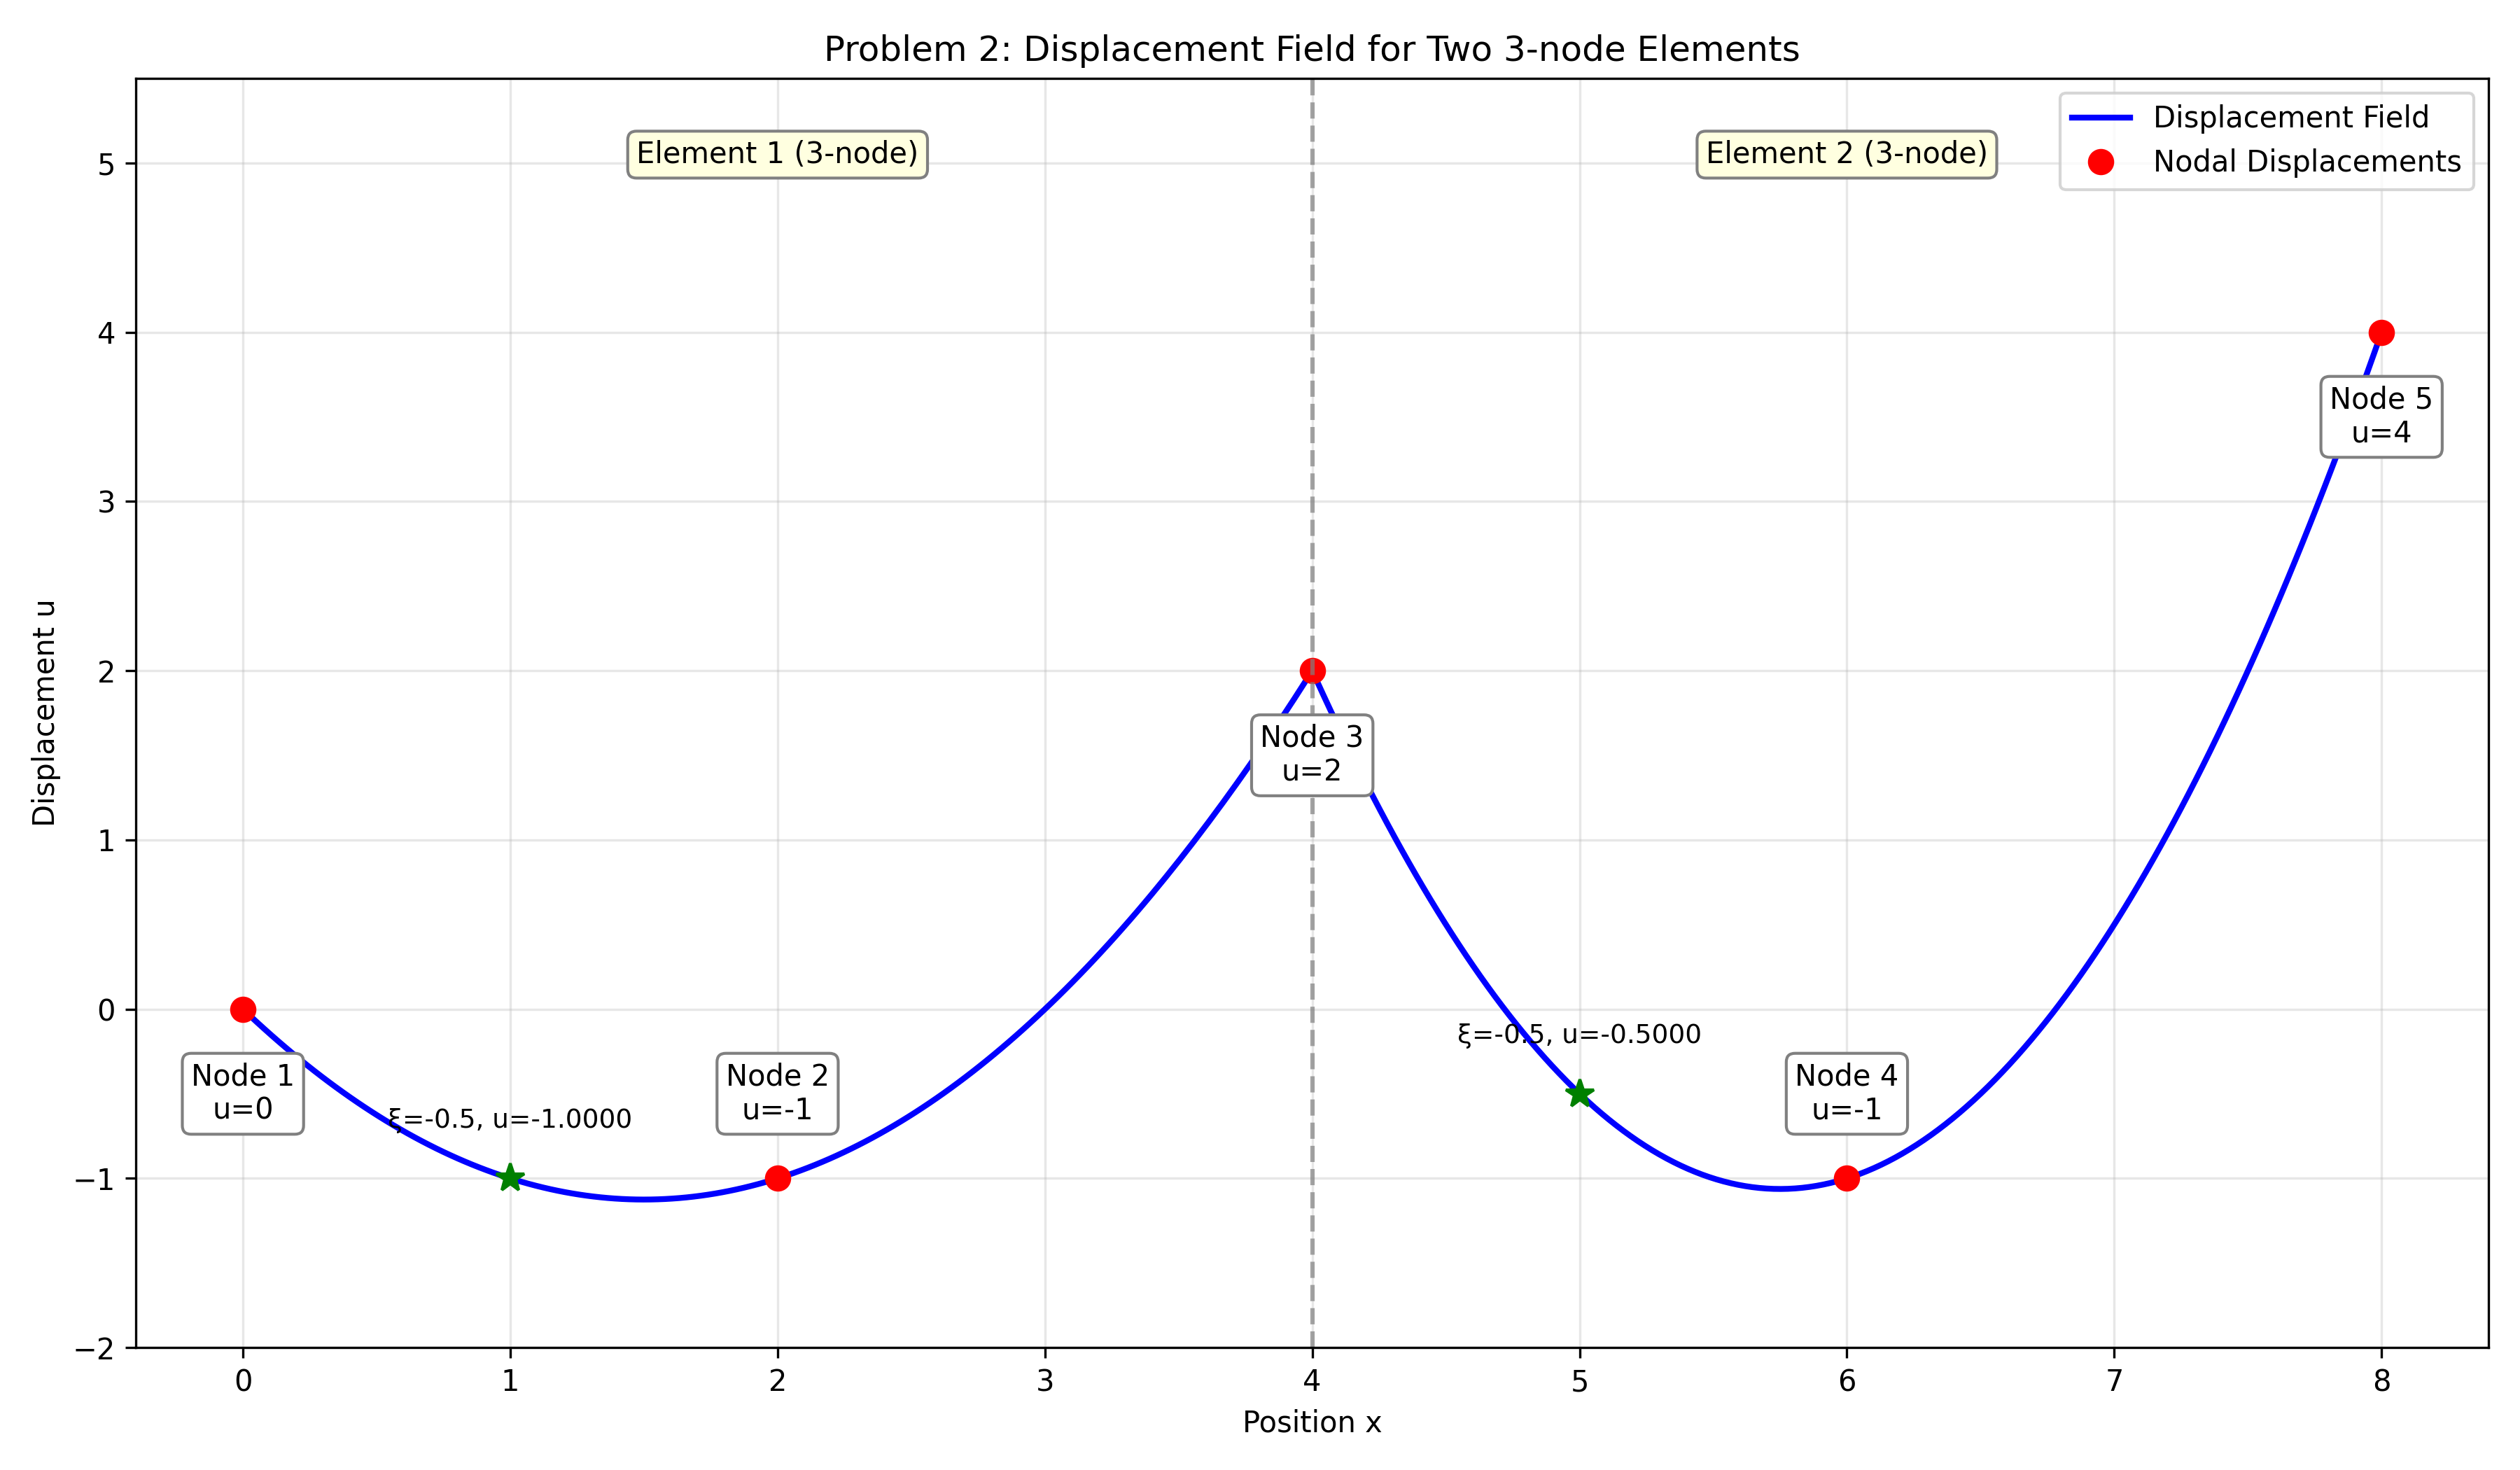
\includegraphics[width=0.8\textwidth]{figures/ps3_problem2_displacement.png}
\caption{Problem 2: Displacement field for the two 3-node elements}
\label{fig:problem2_displacement}
\end{figure}

\subsection{Strains at $\xi = -0.5$}
For 3-node elements, the strain varies within the element and is calculated using:
\begin{equation}
\varepsilon = \mathbf{B} \cdot \mathbf{u}, \text{ where } \mathbf{B} = \left[\frac{dN_1}{dx}, \frac{dN_2}{dx}, \frac{dN_3}{dx}\right]
\end{equation}

At $\xi = -0.5$:
\begin{align}
\frac{dN_1}{d\xi} &= \xi - 0.5 = -0.5 - 0.5 = -1.0 \\
\frac{dN_2}{d\xi} &= -2\xi = -2 \times (-0.5) = 1.0 \\
\frac{dN_3}{d\xi} &= \xi + 0.5 = -0.5 + 0.5 = 0.0
\end{align}

The Jacobian for both elements (L = 4):
\begin{equation}
J = \frac{L}{2} = \frac{4}{2} = 2
\end{equation}

Converting to derivatives with respect to $x$:
\begin{align}
\frac{dN_1}{dx} &= \frac{dN_1}{d\xi} \cdot \frac{d\xi}{dx} = \frac{-1.0}{2} = -0.5 \\
\frac{dN_2}{dx} &= \frac{dN_2}{d\xi} \cdot \frac{d\xi}{dx} = \frac{1.0}{2} = 0.5 \\
\frac{dN_3}{dx} &= \frac{dN_3}{d\xi} \cdot \frac{d\xi}{dx} = \frac{0.0}{2} = 0.0
\end{align}

\subsubsection*{Element 1:}
\begin{align}
\varepsilon &= -0.5 \times 0 + 0.5 \times (-1) + 0.0 \times 2 \\
&= 0 - 0.5 + 0 = -0.5
\end{align}

\subsubsection*{Element 2:}
\begin{align}
\varepsilon &= -0.5 \times 2 + 0.5 \times (-1) + 0.0 \times 4 \\
&= -1.0 - 0.5 + 0 = -1.5
\end{align}

\begin{figure}[H]
\centering
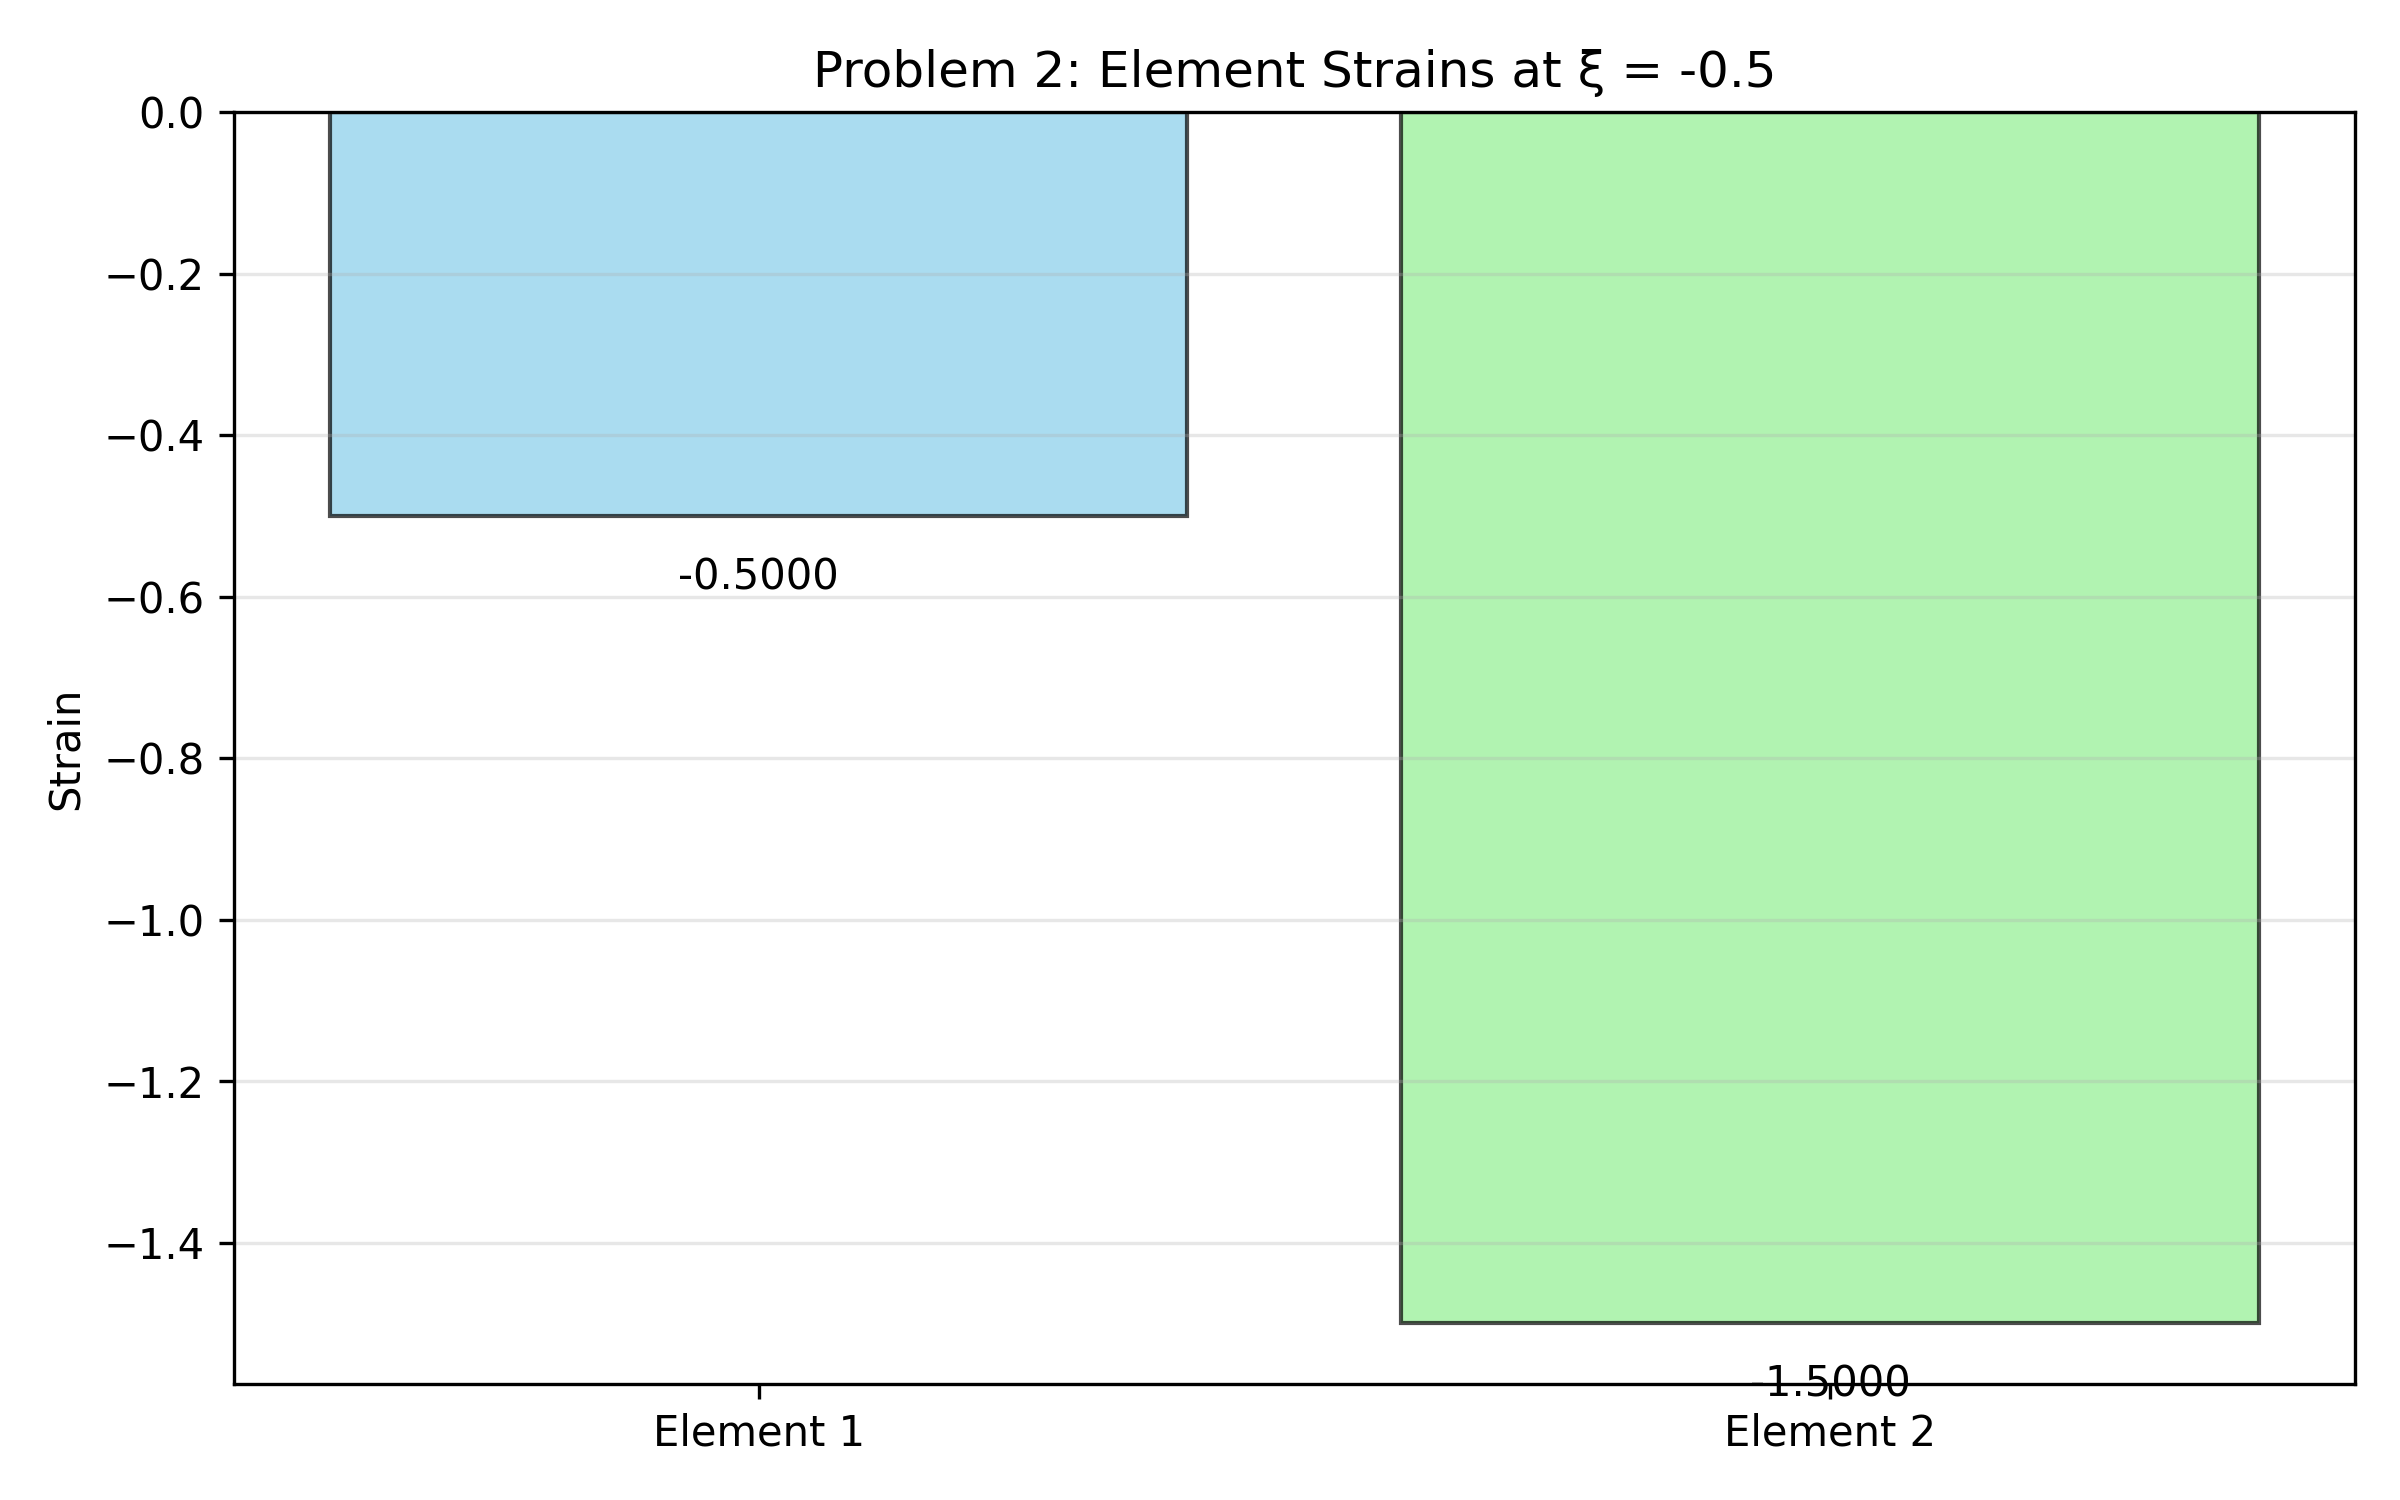
\includegraphics[width=0.8\textwidth]{figures/ps3_problem2_strains.png}
\caption{Problem 2: Element strains for the two 3-node elements}
\label{fig:problem2_strains}
\end{figure}

\subsection{Stiffness Matrices}
For a 3-node element, the stiffness matrix is calculated using numerical integration:
\begin{equation}
\mathbf{k} = \int\mathbf{B}^T \cdot E \cdot \mathbf{B} \cdot A \cdot \det(J) \, d\xi
\end{equation}

Using integration points $\xi = -0.5$ and $\xi = 0.5$ with equal weights of 1.0 and assuming $E = A = 1$:

\begin{figure}[H]
\centering
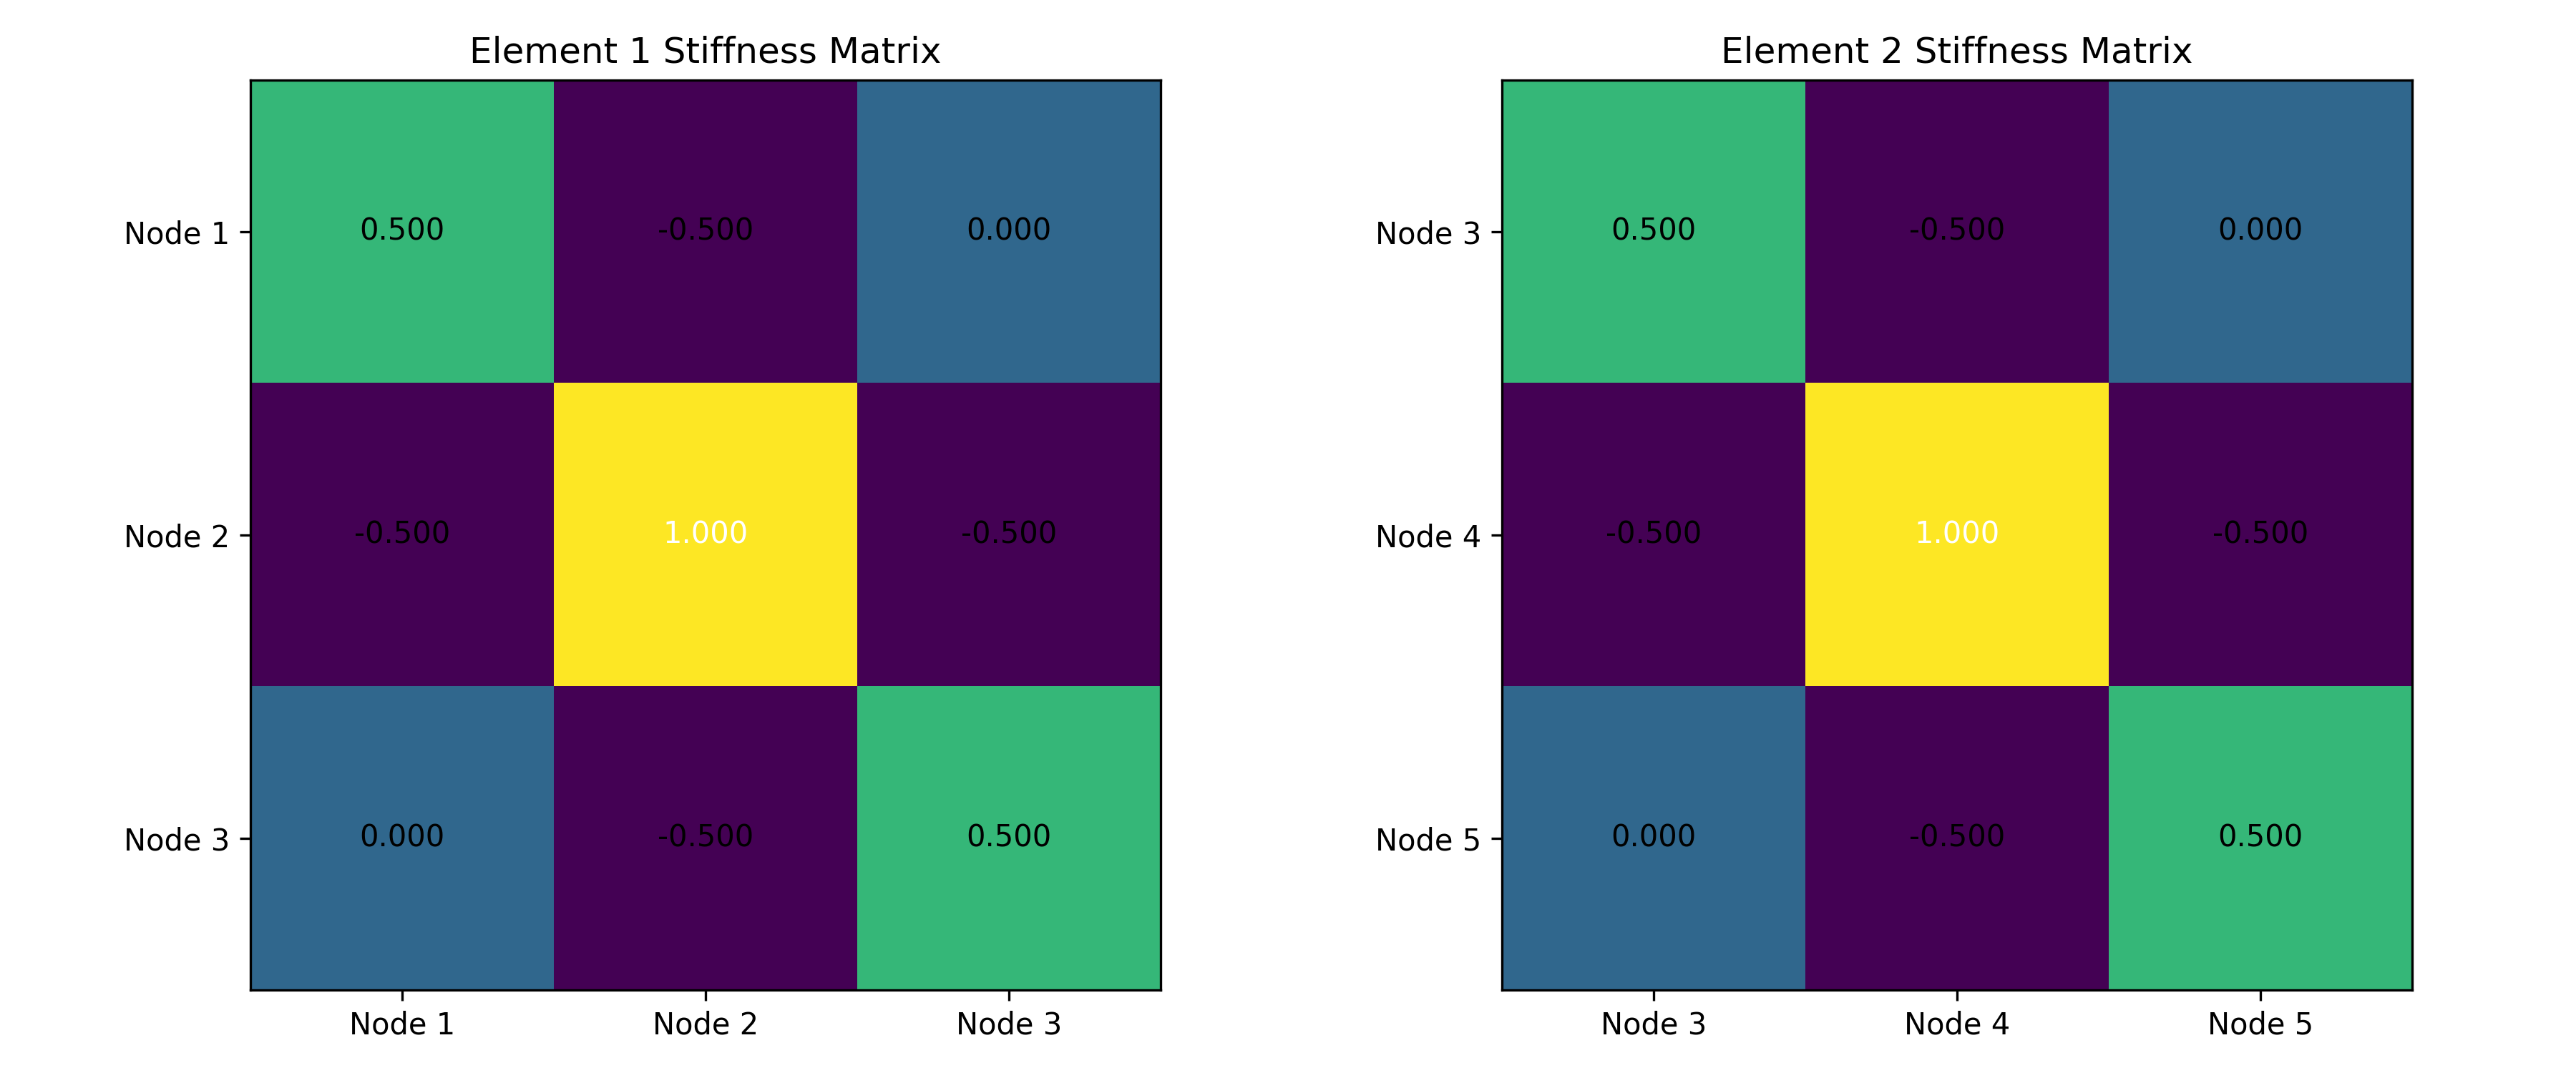
\includegraphics[width=0.8\textwidth]{figures/ps3_problem2_stiffness.png}
\caption{Problem 2: Stiffness matrices for the two 3-node elements}
\label{fig:problem2_stiffness}
\end{figure}

\section{Conclusion}
This report has presented solutions for two finite element problems involving 2-node and 3-node elements. We derived the shape functions, calculated displacements and strains at specific points in the elements, and computed element stiffness matrices using appropriate integration methods. The results demonstrate how the finite element method can effectively model displacement fields and strain distributions in one-dimensional structures.

The analysis of Problem 1 with three 2-node elements showed constant strain within each element, while Problem 2 with two 3-node elements exhibited varying strain distributions. These results align with the theoretical expectations for linear and quadratic elements, respectively.

\end{document}
